\documentclass[aspectratio=169]{beamer}
\usetheme{boxes}
\usepackage{essay-def}
\usepackage{bm}
\usepackage{booktabs}
\usepackage{amsfonts}
\usepackage{amssymb}
\usepackage{amsmath}
\usepackage{amsthm}
\usepackage{comment}
\usepackage{subcaption}
\usepackage{geometry}
\usepackage{algorithmic}
\usepackage{algpseudocode}
\usepackage{algorithmicx}
\usepackage[version=4]{mhchem}
\geometry{left=1cm,right=1cm}
    \title[Gaussian Hartree-Fock]{Adaptive Gaussian basis for quantum chemistry calculation}
\author[J. Zhao]{Jiaxi Zhao (NUS)\\joint work with Doc. Min Lin (SAIL)}
\date[\today]{\today\\
Joint FDU-NUS-ZJU
PhD Forum in Mathematics}
\begin{document}
\par \setlength{\parindent}{2em}

\begin{frame}
\titlepage
\end{frame}

\begin{frame}{What is quantum chemistry?}

	Recall in high school chemistry, we learned:
	\begin{itemize}
		\item 1. Atoms have s, p, d, f, etc orbitals, Pauli exclusion principle, Hund's Rules.
		\item 2. There are ionic and covalent bonds.
		\item 3. Materials can be conductors, semi-conductors, and insulators.
	\end{itemize}

	{\color{red} All these properties can be explained by the electronic structure from
	first principle calculations!}
	
\end{frame}

% for long talk
% \begin{frame}{Many-body Schr\"odinger equation}
% 	After Born–Oppenheimer approximation, the many-body Schr\"odinger equation
% 	is given by:
% 	\begin{equation*}
% 		\begin{aligned}
% 			\hat{\opH^e} & \Psi(\mfr_1, \mfr_2, ..., \mfr_N) = E
% 			\Psi(\mfr_1, \mfr_2, ..., \mfr_N),		\\
% 			\hat{\opH^e} & = -\half \Delta_{\mfr} - \sum_{i=1}^N\sum_{j=1}^{n_A} \frac{Z_j}
% 			{\norml \mfr_i - \mfR_j \normr_2} + \frac{1}{2} \sum_{i \neq j}^N
% 			\frac{1}{r_{ij}}		\\
% 			& = \sum_{i=1}^N \wht{\operatorname{h}}(\text{i}) + \frac{1}{2} \sum_{i \neq j}^N
% 			\frac{1}{r_{ij}}
% 		\end{aligned}
% 	\end{equation*}
% 	Solving this equation, we can obtain the ground state energy, potential
% 	energy surface (for geometry optimization and transition states search),
% 	band structure for the solid state system, and etc.
% \end{frame}

% % for long talk
% \begin{frame}{Mean-field approximation: Slater determinant}
% 	Pauli exclusion principle requires following antisymmetric constraint on the
% 	many-body wave function:
% 	\begin{equation*}
% 		\Psi_{\text{HF}}(..., \mfr_j, ..., \mfr_i, ...) = 
% 		- \Psi_{\text{HF}}(..., \mfr_i, ..., \mfr_j, ...)
% 	\end{equation*}

% 	The many-body wave function of the Hartree-Fock theory is given by a single
% 	Slater determinant:
% 	\begin{equation*}
% 		\Psi_{\text{HF}}(\mfr_1, ..., \mfr_N) = \frac{1}{\sqrt{N!}} 
% 		\begin{vmatrix}
% 			\phi_1(\mfr_1) & \phi_1(\mfr_2) & \cdots & \phi_1(\mfr_N) \\
% 			\phi_2(\mfr_1) & \phi_2(\mfr_2) & \cdots & \phi_2(\mfr_N) \\
% 			\vdots & \vdots & \ddots & \vdots \\
% 			\phi_N(\mfr_1) & \phi_N(\mfr_2) & \cdots & \phi_N(\mfr_N)
% 		\end{vmatrix}
% 	\end{equation*}
% 	{\color{red} This part is still a bit confusing for math audience.}
% \end{frame}

% % for long talk
% \begin{frame}{Total energy}
% 	\begin{equation*}
% 		\begin{aligned} & E[\Psi^{HF}] = 
% 			\left\langle\Psi^{HF}|\hat{\opH^e}|\Psi^{HF}
% 			\right\rangle =  \sum_{i=1}^N \int\text{d}\mathbf{r}_i
% 		  \phi_i^*(\mathbf{r}_i)
% 			\wht{\operatorname{h}}(\text{i}) \phi_i(\mathbf{r}_i) \\ 
% 			&+ \frac{1}{2N(N - 1)} \sum_{i \neq j}^N \sum_{k \neq l}^N \iint
% 			\mathrm{d}\mathbf{r}_i
% 			\text{d}\mathbf{r}_j \phi_k^*(\mathbf{r}_i)\phi_l^*(\mathbf{r}_j)
% 			\frac{1}{|\mathbf{r}_i-\mathbf{r}_j|}\phi_k(\mathbf{r}_i)
% 			\phi_l(\mathbf{r}_j) \\ 
% 			&- \frac{1}{2N(N - 1)} \sum_{i \neq j}^N \sum_{k \neq l}^N \iint
% 			\text{d}\mathbf{r}_i
% 			\text{d}\mathbf{r}_j\phi_k^*(\mathbf{r}_i)\phi_l^*(\mathbf{r}_j)
% 			\frac{1}{|\mathbf{r}_i-\mathbf{r}_j|}\phi_k(\mathbf{r}_j)
% 			\phi_l(\mathbf{r}_i)  \\
% 			& = E(\phi_1, \phi_2, \cdots, \phi_N).
% 		\end{aligned}
% 	\end{equation*}
% 	Minimizing the total energy will give the ground state configuration which is
% 	consistent with the self-consistent field approach. The double-electron
% 	integrations $O(N^4)$ are the dominant part of computational cost.
% \end{frame}

\begin{frame}{Mathematical formulation}
	Variational formulation of the Hartree-Fock theory:
	\begin{equation*}
		\begin{aligned}
			& E(\phi_1, \phi_2, \cdots, \phi_N) = 
	\sum_{i=1}^N \int\text{d}\mathbf{r}_i
		  \phi_i^*(\mathbf{r}_i) (-\frac{1}{2}\Delta - \sum_{\text{atom } a}
			\frac{Z_a}{|\mathbf{r}_i - \mathbf{A}_a|})(\mathbf{r}_i))
			 \phi_i(\mathbf{r}_i) \\ 
			&+ \frac{1}{2N(N - 1)} \sum_{i \neq j}^N \sum_{k \neq l}^N \iint
			\mathrm{d}\mathbf{r}_i
			\frac{1}{|\mathbf{r}_i-\mathbf{r}_j|}
			\left(\underbrace{\phi_l(\mathbf{r}_j)\phi_l^*(\mathbf{r}_j)}_{\rho_l(\mathbf{r}_j)}
			\text{d}\mathbf{r}_j \overbrace{\phi_k^*(\mathbf{r}_i)\phi_k(\mathbf{r}_i)
			}^{\rho_k(\mathbf{r}_i)} - \underbrace{\phi_k^*(\mathbf{r}_i)\phi_l^*(\mathbf{r}_j)
			\phi_k(\mathbf{r}_j)\phi_l(\mathbf{r}_i)}_{\text{Exchange term}}\right)  \\
      & \int\text{d}\mathbf{r}
		  \phi_i^*(\mathbf{r}) \phi_j(\mathbf{r}) = \delta_{ij}.
		\end{aligned}
	\end{equation*}
	\begin{itemize}
		\item 1. Mean-field approximation of the quantum many-body Schr\"odinger equation.
		\item 2. Direct optimization of the total energy; self-consistent field (SCF) method.
		\item 3. Discretization of the wave function: $\phi_j = \sum_{i\in I} c_{ji}\varphi_i$.
	\end{itemize}
\end{frame}

\begin{frame}{Basis set\footnotemark}
	\begin{itemize}
		\item Slater basis functions:
		\begin{equation*}
			\varphi_{a, A, \alpha}^{\opS} \equiv (x - A_x)^{a_x} (y - A_y)^{a_y}
			(z - A_z)^{a_z} e^{-\alpha \norml \mfr - \mfA \normr_2}.
		\end{equation*}
		\item Gaussian basis functions:
		\begin{equation*}
			\varphi_{a, A, \alpha}^{\opG} \equiv (x - A_x)^{a_x} (y - A_y)^{a_y}
			(z - A_z)^{a_z} e^{-\alpha \norml \mfr - \mfA \normr_2^2}.
		\end{equation*}
		\item Contracted Gaussian basis functions (PySCF, QChem):
		\begin{equation*}
			\varphi_{a, A, \alpha, k}^{\text{c}\opG} \equiv \sum_{k=1}^{K_A}
			D_{aAk}(x - A_x)^{a_x}(y - A_y)^{a_y}(z - A_z)^{a_z}
			e^{-\alpha_k \norml \mfr - \mfA \normr_2^2}.
		\end{equation*}
		\item Numerical atomic orbitals (Abacus):
		\begin{equation*}
			\varphi_{a, A, \alpha, k} \equiv \sum_{L}^{L_A}
			Y_L(\widehat{\mathbf{r} - \mathbf{A}})
			f_L(\norml \mathbf{r} - \mathbf{A} \normr_2^2).
		\end{equation*}
	\end{itemize}
	\footnotetext[1]{Gill, Peter MW. "Molecular integrals over gaussian basis
	functions." Advances in quantum chemistry. Vol. 25. Academic Press, 1994.
	141-205.}
\end{frame}

% for long talk
\begin{frame}{A primer on molecular integral over Gaussian basis functions}
	It suffices to evaluate the fundamental integrals:
	\begin{equation*}
		\iint e^{-\alpha \norml \mfr_1 - \mfA \normr_2^2}
		e^{-\beta \norml \mfr_2 - \mfB \normr_2^2} f(r_{12})
		e^{-\gamma \norml \mfr_1 - \mfC \normr_2^2}
		e^{-\delta \norml \mfr_2 - \mfD \normr_2^2}d\mfr_1d\mfr_2.
	\end{equation*}
	Integrations involving higher angular momentum can be calculated by
	taking the derivation w.r.t. $\mfr_1, \mfr_2$ and recursive formula.

	{\color{red}Caveat: the recursive formula becomes very complex for higher
	angular momentum and thus computationally expensive.}
\end{frame}

\begin{frame}{Adaptive Gaussian basis}
	% Classically, basis set of increasing complexity is used to 
	% \begin{itemize}
	% 	\item 1. STO-n 
	% 	\item 2. 6-311G*
	% 	\item 3. cc-pVDZ
	% \end{itemize}

	{\color{red}\textbf{Basis set optimization}} is also a hot topic for research.

	Adaptive Gaussian basis with optimizable mean and covariance:
	\begin{equation*}
		\phi_i = \sum_{j\in I} c_{ij}\mcN(\mfr; \mu_j, \Sigma_j).
	\end{equation*}
	In general, all the optimizable parameters are $\mu \in \mbR^{|I|\times 3},
	\Sigma \in \lp \mbS_+^3 \rp^{|I|}, C \in \mbC^{|I|\times N}$. $|I|$ is the
	size of the basis set, $N$ is the number of electrons.

	\begin{itemize}
		\item 1. More flexibility to model the wave functions.
		\item 2. Analytic Gaussian integral.
	\end{itemize}
	\footnotetext{Kerbl, Bernhard, et al. "3D Gaussian Splatting for Real-Time
	Radiance Field Rendering." ACM Trans. Graph. 42.4 (2023): 139-1.}
\end{frame}

\begin{frame}{Orthonormality and overlap matrix}
	The orthonormality of the orbitals in SCF is guaranteed by the eigensolver.
	In total energy minimization, we have to handle this explicitly.

	As the orbitals are supposed to be orthonormal, it can be written as
	\begin{equation*}
		\opC^{\dagger} \opS \opC = \opI.
	\end{equation*}
	where $\opS$ is the overlap matrix defined as:
	\begin{equation*}
		\operatorname{S}_{ij} = \la \mcN\lp \mfr; \mathbf{\mu_i},
    \Sigma_i \rp \rv \left. \mcN\lp \mfr;
    \mathbf{\mu_j}, \Sigma_j \rp \ra.
	\end{equation*}
	The orthonormality is enforced by QR decomposition modified by the
	Cholesky factorization of $\opS$.
\end{frame}

\begin{frame}{Coulomb and external energy}
	Why difficulites? No analytic formula for
	\begin{equation}
		\la \mcN\lp \mfr_1 | \mathbf{\mu_1}, \Sigma_1 \rp \rv \frac{1}{
				\lv \mfr_1 - \mfr_2 \rv}\lv \mcN\lp \mfr_2 | \mathbf{\mu_2}, \Sigma_2
				\rp \ra
	\end{equation}

	Our primary idea is to approximate the Coulomb kernel by a series of
	Gaussian modes:
	\begin{equation*}
		\frac{1}{r} = \sum_i c_i e^{-\alpha_i r^2},
	\end{equation*}
	which is done by minimizing the following
	\begin{equation*}
		\begin{aligned}
			\min_{c_i, \alpha_i} \int_{B_M} \lp \frac{1}{|\mfr|} - \sum_i c_i
			e^{-\alpha_i |\mfr|^2} \rp^2 d\mfr = 4\pi\int_0^M \lp 1 - \sum_i c_i
			re^{-\alpha_i r^2} \rp^2 dr
		\end{aligned}
	\end{equation*}
	Then we fix the number of Gaussian modes and optimize the analytic loss
	function via gradient-based optimization.
\end{frame}

% for long talk
% \begin{frame}{Analysis of the nonlinear optimization problem}
% 	\begin{equation*}
% 		\begin{aligned}
% 			& \ \int_0^M \lp 1 - \sum_i c_i re^{-\alpha_i r^2} \rp^2 dr 
% 			\overset{u = kr}{=} & \ \frac{1}{k}\int_0^{kM} \lp 1 - \sum_i \frac{c_i}{k} u 
% 			e^{-\frac{\alpha_i}{k^2} u^2} \rp^2 du.
% 		\end{aligned}
% 	\end{equation*}
% 	The optimal solution for different $M$ can be obtained by rescaling the optimal
% 	coefficient and variance of the Gaussian modes.

% 	However, optimizing such problem to a relatively low threshold, e.g. $10^{-5}$
% 	is quite difficult.
% 	\begin{figure}[h]
% 		\centering
% 		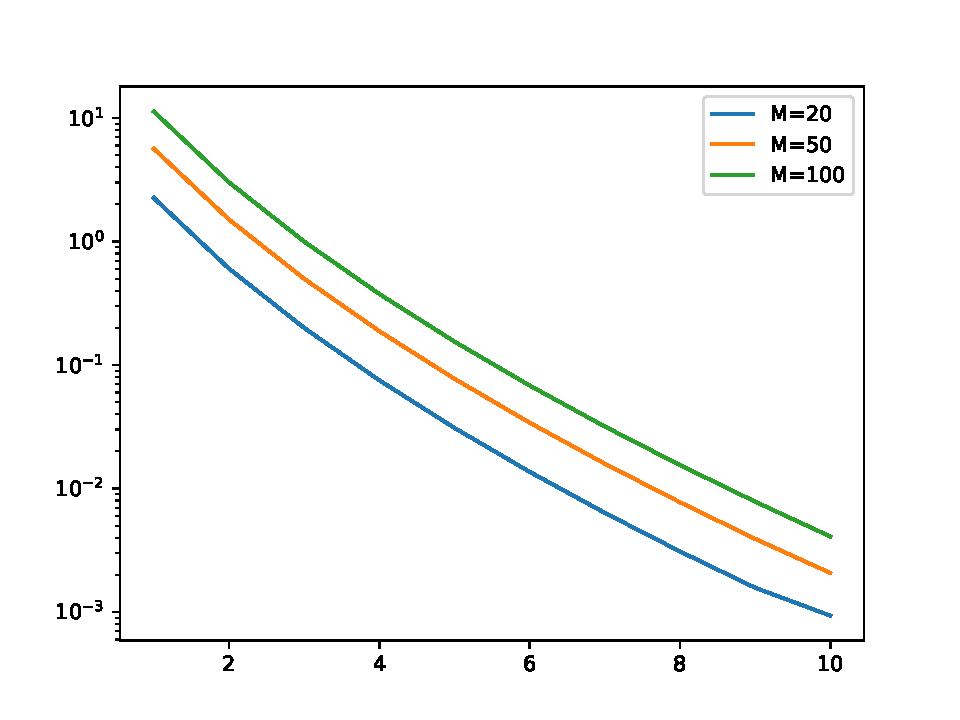
\includegraphics[width=0.5\linewidth]{fig/convergence.pdf}
% 	\end{figure}
% \end{frame}

\begin{frame}{Coulomb kernel decomposition}
	\begin{figure}[h]
		\centering
		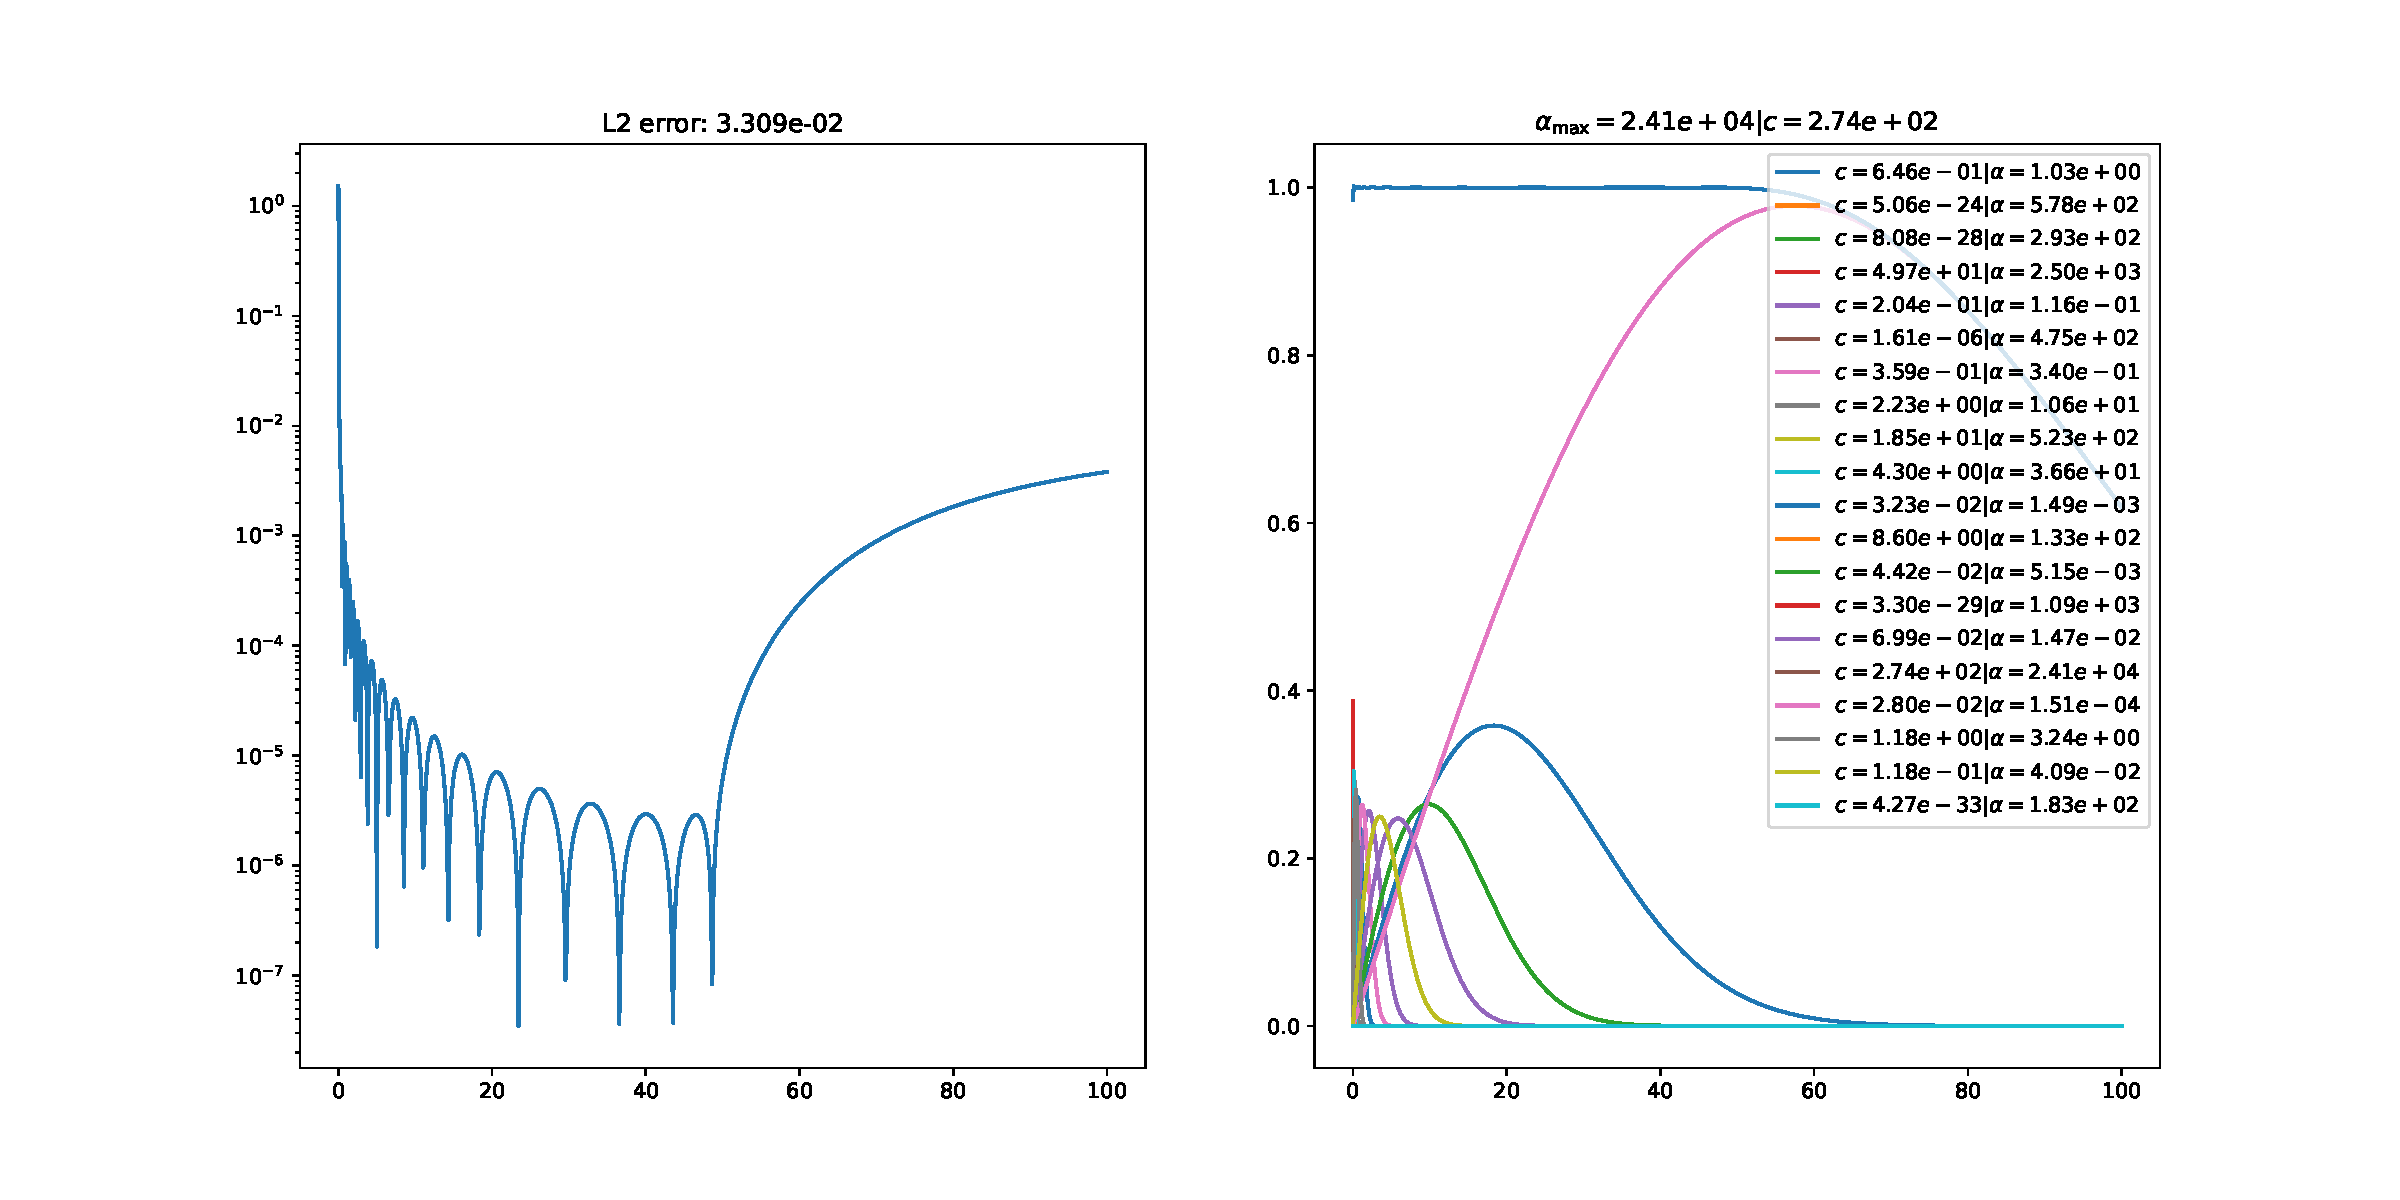
\includegraphics[width=\linewidth]{fig/modes_M50i20.pdf}
	\end{figure}
\end{frame}

\begin{frame}{More on double electron integrals}
	\begin{equation*}
		\begin{aligned}
			& \ \la \mcN\lp \mfr_1 | \mathbf{\mu_1}, \Sigma_1 \rp \rv \frac{1}{
				\lv \mfr_1 - \mfr_2 \rv}\lv \mcN\lp \mfr_2 | \mathbf{\mu_2}, \Sigma_2
				\rp \ra     \\
			= & \ \int\int d\mfr_1d\mfr_2 \frac{1}{\sqrt{(2\pi)^6\det(\Sigma_1)
			\det(\Sigma_2)}} \sum_i c_i  \exp\lb -\half\lp (\mfr_1 - \mu_1)^T
			\Sigma_1^{-1}(\mfr_1 - \mu_1) \right.\right.		\\
				& \ \left.\left. + (\mfr_2 - \mu_2)^T\Sigma_2^{-1}(\mfr_2 - \mu_2)\rp
				- (\mfr_1 - \mfr_2)^T \alpha_i \operatorname{I} (\mfr_1 - \mfr_2) \rb
			\\
			= & \ \int\int d\mfr \frac{\sum_i c_i s(i)\exp\lb -\half(\mfr - \mu(i))^T \begin{pmatrix}
				\Sigma_1^{-1} + 2\alpha_i \operatorname{I} & -2\alpha_i \operatorname{I}
				\\
				-2\alpha_i \operatorname{I} & \Sigma_2^{-1} + 2\alpha_i \operatorname{I}
				\end{pmatrix} (\mfr - \mu(i)) \rb}{\sqrt{(2\pi)^6\det(\Sigma_1)
			\det(\Sigma_2)}}.
		\end{aligned}
	\end{equation*}
	\begin{itemize}
		\item 1. solving a linear system of size $3\times 3$, MVP of size $3\times 3$, calculating
		the determinant of a $3\times 3$ matrix.
		\item 2. The FLOPs count for a single ERI evaluation with one $\alpha$ is around 60, comparing
		to classical method: (ss|ss), (ps|ps), (pp|pp) requires 33, 58, 1326 FLOPs for a single evaluation.
	\end{itemize}
\end{frame}

\begin{frame}{Parameterization of Gaussian basis}
	We parameterize the Gaussian basis as
	\begin{equation*}
		\Sigma_1 = \opU_1 \opD_1 \opU_1^T, \quad \Sigma_2 = \opU_2 \opD_2 \opU_2^T,
	\end{equation*}
	where $\opU_i$ is obtained from the QR decomposition and the positivity of
	the diagonal element of $\opD_i$ is enforced by the softplus function.

	This is proved to be more robust than parametrization by Cholesky
	factorization.
\end{frame}

\begin{frame}{Numerical experiments}
	\begin{table}[tb]\label{table:accuracy-2d-ot}
		\label{table:density-fitting}
		\centering
		\Large
		\resizebox{0.95\columnwidth}{!}{
		\begin{tabular}{P{4cm} P{2cm} P{2cm} P{2cm} P{2cm} P{2cm} P{2cm} P{2cm}}
		\toprule [1.5pt]
		\parbox{4cm}{  } &   \parbox{2cm}{ \centering e\_kin + e\_ext} &
		\parbox{2cm}{\centering  e\_kin}
		& \parbox{2cm}{\centering  e\_ext} & 
		\parbox{2cm}{ \centering e\_nuc } & \parbox{2cm}{ \centering 
		e\_coul + e\_exc} & \parbox{2cm}{ \centering 
		e\_coul} & \parbox{2cm}{ \centering e\_exc} & \parbox{2cm}
		{\centering  e\_tot}   \\ \midrule[1.5pt]
		
		\parbox{4cm}{OUR ($\ce{H2}$), 10} & -2.5062 & 1.1254 & -3.6316 & 0.7138 & 0.6591 &
		1.3182 & -0.6591 & \textbf{-1.1334} \\ \midrule[0.5pt]
	
		% \parbox{3cm}{$n_g= 10, \epsilon=10^{-3}$} & -2.4905 & 1.1070 & -3.5975
		% & 0.7138 & 0.6549 & 1.3097 & -0.6549 & -1.1219 \\ \midrule[0.5pt]
	
		% \parbox{3cm}{$n_g = 20, \epsilon=10^{-3}$} & -2.4897 & 1.1069 & -3.5966
		% & 0.7138 & 0.6547 & 1.3094 & -0.6547 & -1.1213 \\ \midrule[0.5pt]
	
		% \parbox{3cm}{$n_g = 20, \epsilon=10^{-4}$} & -2.4917 & 1.1095 & -3.6012
		% & 0.7138 & 0.6550 & 1.3100 & -0.6550 & -1.1229 \\ \midrule[0.5pt]
	
		% \parbox{3cm}{$n_g = 10, \epsilon=10^{-4}$} & -2.4909 & 1.1078 & -3.5987
		% & 0.7138 & 0.6550 & 1.3100 & -0.6550 & -1.1221 \\ \midrule[0.5pt]
	
		\parbox{4cm}{HF (STO-3G, 2)} 
		& -2.5049 &  * & * & 0.7138 & 0.6745 & * & * & -1.1167
		\\ \midrule[0.5pt]
	
		\parbox{4cm}{HF (6-31G, 4)} 
		& -2.4902 &  * & * & 0.7138 & 0.6497 & * & * & -1.1267
		\\ \midrule[0.5pt]
	
		\parbox{4cm}{HF (6-311G, 6)} 
		& -2.4924 &  * & * & 0.7138 & 0.6507 & * & * & \textbf{-1.1280}
		\\ \midrule[0.5pt]
	
		% \parbox{3cm}{d4ft (6-31g, lda)} 
		% & -2.482366 & * & * & 0.713754 & * & 1.280327 & -0.552556 & -1.038646
		% \\ \midrule[0.5pt]
	
		% \parbox{3cm}{pyscf} 
		% & -2.480171 & * & * & 0.713754 & * & 1.275792 & -0.554381 & -1.047201
		% \\ \midrule[0.5pt] \midrule[0.5pt]
	
		% \parbox{3cm}{OUR (\ce{CH4})} & -78.6437 & 37.8278 & -116.4715 & 13.4477
		% & 25.8757 & 32.3750 & -6.4993 & -39.3203 \\ \midrule[0.5pt]
	
		% \parbox{3cm}{$n_g = 10, \epsilon=10^{-3}$} & -78.3927 & 39.6854 &
		% -118.0781 & 13.4477 & 25.6199 & 32.2481 &
		% -6.6282 & -39.3251 \\ \midrule[0.5pt]
	
		% \parbox{3cm}{$n_g = 20, \epsilon=10^{-3}$} & -79.3790 & 39.9992 &
		% -119.3782 & 13.4477 & 26.01440 & 32.5979 &
		% -6.5835 & -39.9169 \\ \midrule[0.5pt]
	
		% \parbox{3cm}{$n_g = 20, \epsilon=10^{-4}$} & -79.2670 & 39.8448 &
		% -119.1118 & 13.4477 & 25.9379& 32.5050 &
		% -6.5671 & -39.8813 \\ \midrule[0.5pt]
	
		% \parbox{3cm}{$n_g = 10, \epsilon=10^{-4}$} & -77.5650 & 39.5177 &
		% -117.0827 & 13.4477 & 24.9640 & 31.5523 &
		% -6.5883 & -39.1532 \\ \midrule[0.5pt]
	
		\parbox{4cm}{OUR ($\ce{CH4}$), 22} & -79.6713 & 40.0987 & -119.7700 & 13.4477
		& 26.1010 & 32.6936 & -6.5926 & \textbf{-40.1225} \\ \midrule[0.5pt]
	
		\parbox{4cm}{HF (STO-3G, 9)} 
		& -79.3617 &  * & * & 13.4477 & 26.1872 & * & * & -39.7267
		\\ \midrule[0.5pt]
	
		\parbox{4cm}{HF (6-31G, 17)} 
		& -79.6901 &  * & * & 13.4477 & 26.0619 & * & * & \textbf{-40.1804}
		\\ \midrule[0.5pt]
	
		\parbox{4cm}{HF (6-311G, 25)} 
		& -79.6872 &  * & * & 13.4477 & 26.0515 & * & * & -40.1880
		\\ \midrule[0.5pt]
	
		% \parbox{3cm}{d4ft} 
		% & -79.503407 & * & * & 13.349528 & * & 32.452280 & -5.856054 & -39.467655
		% \\ \midrule[0.5pt]
	
		% \parbox{3cm}{pyscf} 
		% & -79.472583 & * & * & 13.349528 & * & 32.586078 & -5.843392 & -39.290969
		% \\ \midrule[0.5pt] \midrule[0.5pt]
	
		% \parbox{3cm}{OUR (\ce{H2O})} & -120.2329 & 68.1350 & -188.3679 & 9.1895 &
		% 37.4786 & 46.2207 & -8.7421 & -73.5648 \\ \midrule[0.5pt]
	
		% \parbox{3cm}{$n_g = 10, \epsilon=10^{-3}$} & -120.9352 & 74.8185 &
		% -195.7537 & 9.1895 & 37.0497 & 46.0144 &
		% -8.9647 & -74.6960 \\ \midrule[0.5pt]
	
		% \parbox{3cm}{$n_g = 20, \epsilon=10^{-3}$} & -122.6473 & 75.5681 &
		% -198.2154 & 9.1895 & 37.7575 & 46.6995 &
		% -8.9420 & -75.7003 \\ \midrule[0.5pt]
	
		% \parbox{3cm}{$n_g = 20, \epsilon=10^{-4}$} & -122.7171 & 75.8241 &
		% -198.5412 & 9.1895 & 37.8074 & 46.7600 &
		% -8.9526 & -75.7202 \\ \midrule[0.5pt]
	
		% \parbox{3cm}{$n_g = 10, \epsilon=10^{-4}$} & -119.5637 & 74.4819 &
		% -194.0456 & 9.1895 & 36.1289 & 45.0722 &
		% -8.9433 & -74.2454 \\ \midrule[0.5pt]
	
		\parbox{4cm}{OUR ($\ce{H2O}$), 22} & -122.9802 & 75.9462 &
		-199.0371 & 9.1895 & 37.8786 & 46.8579 &
		-8.9601 & \textbf{-76.0036} \\ \midrule[0.5pt]
	
		\parbox{4cm}{HF (STO-3G, 7)} 
		& -122.3614 &  * & * & 9.1895 & 38.2089 & * & * & -74.9630
		\\ \midrule[0.5pt]
	
		\parbox{4cm}{HF (6-31G, 13)} 
		& -122.9701 &  * & * & 9.1895 & 37.7966 & * & * & -75.9839
		\\ \midrule[0.5pt]
	
		\parbox{4cm}{HF (6-311G, 19)} 
		& -123.0146 &  * & * & 9.1895 & 37.8157 & * & * & \textbf{-76.0094}
		\\ \midrule[0.5pt]
	
		% \parbox{3cm}{d4ft} 
		% & -122.983359 & * & * & * & 9.189533 & 46.449287 & -8.117571 & -75.462110
		% \\ \midrule[0.5pt]
	
		% \parbox{3cm}{pyscf} 
		% & -122.839414 & * & * & * & 9.189534 & 46.589372 & -8.093291 & -75.153800
		% \\ \midrule[0.5pt]
	
		\\\bottomrule[1.5pt]
		\end{tabular}
		}
	\end{table}
\end{frame}

\begin{frame}
	Thank you for your attention!
	Q \& A
\end{frame}

\begin{frame}{Many-body Schr\"odinger equation}
	After Born–Oppenheimer approximation, the many-body Schr\"odinger equation
	is given by:
	\begin{equation*}
		\begin{aligned}
			\hat{\opH^e} & \Psi(\mfr_1, \mfr_2, ..., \mfr_N) = E
			\Psi(\mfr_1, \mfr_2, ..., \mfr_N),		\\
			\hat{\opH^e} & = -\half \Delta_{\mfr} - \sum_{i=1}^N\sum_{j=1}^{n_A} \frac{Z_j}
			{\norml \mfr_i - \mfR_j \normr_2} + \frac{1}{2} \sum_{i \neq j}^N
			\frac{1}{r_{ij}}		\\
			& = \sum_{i=1}^N \wht{\operatorname{h}}(\text{i}) + \frac{1}{2} \sum_{i \neq j}^N
			\frac{1}{r_{ij}}
		\end{aligned}
	\end{equation*}
	Solving this equation, we can obtain the ground state energy, potential
	energy surface (for geometry optimization and transition states search),
	band structure for the solid state system, and etc.
\end{frame}

% for long talk
\begin{frame}{Mean-field approximation: Slater determinant}
	Pauli exclusion principle requires following antisymmetric constraint on the
	many-body wave function:
	\begin{equation*}
		\Psi(..., \mfr_j, ..., \mfr_i, ...) = 
		- \Psi(..., \mfr_i, ..., \mfr_j, ...)
	\end{equation*}

	The many-body wave function of the Hartree-Fock theory is given by a single
	Slater determinant:
	\begin{equation*}
		\Psi_{\text{HF}}(\mfr_1, ..., \mfr_N) = \frac{1}{\sqrt{N!}} 
		\begin{vmatrix}
			\phi_1(\mfr_1) & \phi_1(\mfr_2) & \cdots & \phi_1(\mfr_N) \\
			\phi_2(\mfr_1) & \phi_2(\mfr_2) & \cdots & \phi_2(\mfr_N) \\
			\vdots & \vdots & \ddots & \vdots \\
			\phi_N(\mfr_1) & \phi_N(\mfr_2) & \cdots & \phi_N(\mfr_N)
		\end{vmatrix}
	\end{equation*}
\end{frame}

% for long talk
\begin{frame}{Total energy}
	\begin{equation*}
		\begin{aligned} & E[\Psi^{\text{HF}}] = 
			\left\langle\Psi^{\text{HF}}|\hat{\opH^e}|\Psi^{\text{HF}}
			\right\rangle =  \sum_{i=1}^N \int\text{d}\mathbf{r}_i
		  \phi_i^*(\mathbf{r}_i)
			\wht{\operatorname{h}}(\text{i}) \phi_i(\mathbf{r}_i) \\ 
			&+ \frac{1}{2N(N - 1)} \sum_{i \neq j}^N \sum_{k \neq l}^N \iint
			\mathrm{d}\mathbf{r}_i
			\text{d}\mathbf{r}_j \phi_k^*(\mathbf{r}_i)\phi_l^*(\mathbf{r}_j)
			\frac{1}{|\mathbf{r}_i-\mathbf{r}_j|}\phi_k(\mathbf{r}_i)
			\phi_l(\mathbf{r}_j) \\ 
			&- \frac{1}{2N(N - 1)} \sum_{i \neq j}^N \sum_{k \neq l}^N \iint
			\text{d}\mathbf{r}_i
			\text{d}\mathbf{r}_j\phi_k^*(\mathbf{r}_i)\phi_l^*(\mathbf{r}_j)
			\frac{1}{|\mathbf{r}_i-\mathbf{r}_j|}\phi_k(\mathbf{r}_j)
			\phi_l(\mathbf{r}_i)  \\
			& = E(\phi_1, \phi_2, \cdots, \phi_N).
		\end{aligned}
	\end{equation*}
	Minimizing the total energy will give the ground state configuration which is
	consistent with the self-consistent field approach. The double-electron
	integrations $O(N^4)$ are the dominant part of computational cost.
\end{frame}

\begin{frame}{SCF}
	Self-consistent field approach to HF: adding Lagrangian multiplier
	(molecular orbital energy) and the KKT condition translates to an eigenvalue
	problem:
	\begin{equation*}
		\begin{aligned}
			\delta E[\phi_k^*(x_k)] & \ = \delta E(\phi_1, \phi_2, \cdots, \phi_N)
			- \delta\left[\sum_{i=1}^N \sum_{j=1}^N
			\lambda_{ij} \left( \left\langle\phi_i, \phi_j\right\rangle - \delta_{ij}
			\right)\right]		\\
			\wht \opF(\text{k})\phi_k(\mathbf{r}_k) & \equiv \left[ \hat{h}
			(\text{k}) + \hat{J}(\text{k}) - \hat{K}(\text{k}) \right]
			\phi_k(\mathbf{r}_k) = \epsilon_k \phi_k(\mathbf{r}_k),	\\
			\wht \opJ(\text{k}) & \equiv \sum_{j=1}^N \int \mathrm{d}\mathbf{r}_j
			\frac{\phi_j^*(\mathbf{r}_j) \phi_j(\mathbf{r}_j)}{|\mathbf{r}_k-
			\mathbf{r}_j|}= \sum_{j=1}^N \int \mathrm{d}\mathbf{r}_j \frac{\rho(
			\mathbf{r}_j)}{|\mathbf{r}_k-\mathbf{r}_j|},\\
			\wht \opK(\text{k})\phi_{k}(\mathbf{r}_k) & \equiv  \sum_{j=1}^N
			\phi_{j}(\mathbf{r}_k) \int \text{d}\mathbf{r}_j \frac{\phi_j^*
			(\mathbf{r}_j) \phi_k(\mathbf{r}_j)}{|\mathbf{r}_k-\mathbf{r}_j|}.\\
		\end{aligned}
	\end{equation*}
\end{frame}

\begin{frame}{Potential improvement}
	\begin{itemize}
		\item 1. Using greedy algorithm to optimize for more Gaussian modes, i.e.
		one can use the optimization results for less modes as the warm-start
		for more modes.
		\item 2. The approximation interval $[0, M]$ can be done adaptively according
		to the relative position of two Gaussian modes.
		\item 3. Motivated by the Boys function, can we design other decomposition
		of the Coulomb kernel?
		\begin{equation*}
			\frac{1}{r} = C\int_{\mbR} e^{-r^2t^2} dt.
		\end{equation*}
	\end{itemize}
\end{frame}

\begin{frame}{Motivation}
	The effect cutoff used by the plane-wave method to solve large system is
	unaffordable. Moreover, given the nature of the electron density which will
	be concentrated around the nucleus, while away from the nucleus which is the
	case of majority of the computational region, the electron density is
	relatively smooth, the plane-wave method is not efficient.
	\JX{We need to survey the literature for some multiscale basis such as
	the wavelet basis.}

\end{frame}

\begin{frame}{Literature}
	In literature, there has been lots of work on exploring the adaptive basis for
	solving DFT. 
	\begin{itemize}
		\item Use fixed analytic transformation mapping depending on the position of the
		atom. (Similar to the r type mesh refinement in numerical PDE.)
		\item Solve some OT-type problems to predetermine the basis before the SCF
		loop.
	\end{itemize}
	However, our method is different from the above method in several aspects:
	\begin{itemize}
		\item Our basis is continuously optimized during the optimization porcess of
		DFT.
		\item We use Monte-Carlo method to estimate the density related energy,
		differs from the traditional PDE solving method.
	\end{itemize}
\end{frame}

\begin{frame}{Advantages}
	There are several advantages of using the distorted plane-wave method.
	\begin{itemize}
		\item The orthonormality of the basis is preserved.
		\item Calculation of the density related energy can be estimated 
		efficiently by the Monte-Carlo method instead of solving the PDE.
	\end{itemize}
\end{frame}

\begin{frame}{Next step}
	\begin{itemize}
		\item 1. Compare the scalability of the double-electron integral
		calculation over the number of basis functions with the SOTA method, e.g.
		MD, HGP(OS), Rys.
		\item 2. Conduct numerical experiments to check if the adaptive
		Gaussian basis can achieve the same accuracy with a smaller number of
		basis.
		\item 3. Implement post HF method, e.g. CCSD, CCSD(T).
	\end{itemize}
\end{frame}


\begin{frame}{Another attempt: combining normalizing flow with plane-wave calculation}
	
\end{frame}


\begin{frame}{MLXC under the PAW formulation}
	\textbf{\color{red} Why do we need the PAW's formulation?}
\end{frame}

% \begin{frame} % Use [allowframebreaks] to allow automatic splitting across slides if the content is too long
%     \frametitle{References}
 
%     \begin{thebibliography}{99} % Beamer does not support BibTeX so references must be inserted manually as below, you may need to use multiple columns and/or reduce the font size further if you have many references
%         \footnotesize % Reduce the font size in the bibliography
 
% 		\bibitem[migbs]{migbs}
% 		Gill, Peter MW.
% 		\newblock Molecular integrals over gaussian basis functions.
% 		\newblock \emph{Advances in quantum chemistry. Vol. 25. Academic Press,
% 		1994. 141-205.}

% 		\bibitem[3dgs]{3dgs}
% 		Kerbl, Bernhard, et al
% 		\newblock 3D Gaussian Splatting for Real-Time Radiance Field Rendering
% 		\newblock \emph{ACM Trans. Graph. 42.4 (2023): 139-1.}

% 		\bibitem[S.A. and Q.L., 2024]{nigbms}
% 		S. Arisaka and Q. Li (2024)
% 		\newblock Accelerating Legacy Numerical Solvers by Non-intrusive Gradient-based Meta-solving
% 		\newblock \emph{International Conference on Machine Learning 2024}
 
        
%     \end{thebibliography}
% \end{frame}

\end{document}